\chapter{\LaTeX Base}
\section{Hello World in \LaTeX}

\lstset{language=TeX}
\begin{lstlisting}
  \documentclass[a4paper,11pt]{article} % specify the document class, different class for different purpose.
  \begin{document}
  \title{Example}
  \author{Mike Chyson}
  \date{Thu Jan  3 16:22:11 CST 2019}
  \maketitle                    % make a title according to the title and author etc.
  \section{What's this?}        
  This is simple document. It contains a title and a section with text.
  \end{document}
\end{lstlisting}

The output is as follows:
%% 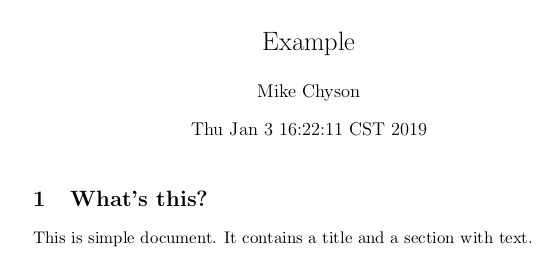
\includepdf[frame=true]{example}
\begin{figure}
  \centering
  \fbox{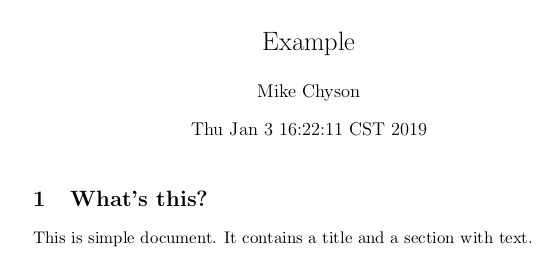
\includegraphics[width=0.8\textwidth]{example.png}}
  \caption{Example}
\end{figure}



Because the seperation of the format and the content, 
you do not specify the font size, font color, font family and so on.
Instead, you tell \LaTeX it is a \lcmd{title}, or \lcmd{author} or \lcmd{date} and so on.
\LaTeX format them for you.
As if there is a logical layer between the appearance and the content.


\section{Document Structure}
A \LaTeX document doesn't stand alone — commonly the document is based on a versatile template.
Such a fundamental template is called a class.
It provides customizable features, usually built for a certain purpose.

This first part of the document is called the preamble of the document. This is where we choose the class, specify properties, and in general, make document-wide definitions.

The first line starts with \verb|\documentclass|.
This word begins with a backslash; such a word is called a \keyword{command}.
We used commands to specify the class and to state document properties: \lcmd{title} , \lcmd{author} , and \lcmd{date}.


\begin{verbatim}
  preamble
  body
\end{verbatim}


\section{\LaTeX Command}
\lstset{language=TeX}
\begin{lstlisting}
  \command
  \command{argument}
  \command[optional argument]{argument}
\end{lstlisting}


\section{Comment}
The percent sing(\%) introduces a \keyword{comment}.




\section{Create Your Own Commands}

\subsection{With No Arguments}
\begin{lstlisting}
  \newcommand{\TUG}{TeX Users Group}
  \TUG
\end{lstlisting}

\subsection{With Arguments}

\begin{lstlisting}
  \newcommand{\keyword}[1]{\textbf{#1}}
  \keyword{declrations}
\end{lstlisting}

\subsection{With Optional Arguments}

\begin{lstlisting}
  \newcommand{\keyword2}[2][\bfseries]{{#1#2}}
  \keyword2[\itshape]{declarations}
\end{lstlisting}


\section{Breaking Lines}
\begin{lstlisting}
  \\                            % end a line
  \newline                      % has the same effect with \\
  \linebreak                    % tells LeTeX to end the line but to keep the full justification
  \\[3mm]                       % insert additional vertical space after the break depending on the value
  \linebreak[4]                 % can be used to influence the line break slightly or strongly:
%% If number is 0, a line break is allowed, 1 means it's desired, 2 and 3 mark more
%% insistent requests, and 4 will force it. The latter is the default behavior if no number
  %% was given.
  \nolinebreak
\end{lstlisting}


\section{Breaking Pages}
\begin{lstlisting}
  \pagebreak
  \newpage
  \nopagebreak
\end{lstlisting}


\section{Get Help}
Three ways to get help about the package:
\begin{itemize}
\item Use the \verb|texdoc| command:
  \begin{lstlisting}
    texdoc <package>
  \end{lstlisting}
\item Use the \verb|kpsewhich| command:
  \begin{lstlisting}
    kpsewhich <package>.sty
  \end{lstlisting}
\item Visit the website: \url{http://ctan.org/pkg}
\end{itemize}
